\documentclass[11pt,a4paper]{article}
\usepackage[margin=0.9in]{geometry}
\usepackage[T1]{fontenc}
\usepackage[utf8]{inputenc}
\usepackage[draft]{graphicx}
\usepackage{hyperref}
\usepackage{enumitem}
\usepackage{float}
\usepackage{amsmath}

\title{Advanced Image Processing Methods\\Homework 4 Report}
\author{Peter Dobosi}
\date{\today}

\begin{document}
\maketitle

\section*{Goal}
Estimate a relative depth (disparity) map from an uncalibrated stereo image pair using fundamental matrix estimation, uncalibrated rectification, and Semi-Global Block Matching.

\section*{Method}
\begin{enumerate}[leftmargin=*,itemsep=2pt]
    \item \textbf{Image Loading}: Both views ($1920\times1080$) are loaded as grayscale with \texttt{cv2.imread}.

    \item \textbf{Keypoint Detection \& Matching}: SIFT is used for detection --- its 128-D float descriptors yield more accurate sub-pixel matches than ORB, which is important since fundamental matrix quality depends directly on match accuracy.
    Descriptors are matched via FLANN (KD-Tree), filtered with Lowe's ratio test ($0.75$), and sorted by ascending distance. Matched $(x,y)$ coordinates are returned as \texttt{float32} arrays.

    \item \textbf{Fundamental Matrix}: Estimated with \texttt{cv2.findFundamentalMat} (\texttt{FM\_RANSAC}, threshold $3.0$, confidence $0.99$). The returned mask is used to keep only inlier point pairs.

    \item \textbf{Rectification}: \texttt{cv2.stereoRectifyUncalibrated} computes homographies $H_L, H_R$ that align epipolar lines horizontally. Both images are warped with \texttt{cv2.warpPerspective}. Black border regions from uncalibrated rectification are expected and handled by SGBM.

    \item \textbf{Disparity (SGBM)}: Computed with \texttt{cv2.StereoSGBM\_create} (parameters in Table~\ref{tab:sgbm}). The raw \texttt{int16} output (scaled by 16) is normalised to $[0,255]$ \texttt{uint8}.

    \item \textbf{Visualisation}: A $1\times3$ Matplotlib figure shows the rectified pair and the colormapped disparity map (brighter $\approx$ closer).
\end{enumerate}

\begin{table}[H]
\centering\small
\begin{tabular}{l|l|l}
    \textbf{Parameter} & \textbf{Value} & \textbf{Reasoning} \\
    \hline
    \texttt{minDisparity}      & $0$    & Standard left-as-reference. \\
    \texttt{numDisparities}    & $128$  & Wide depth range; divisible by 16. \\
    \texttt{blockSize}         & $5$    & Sharp depth edges; smoothness term compensates. \\
    \texttt{P1}                & $200$  & $8 \cdot 1 \cdot 5^2$; small disparity change penalty. \\
    \texttt{P2}                & $800$  & $32 \cdot 1 \cdot 5^2$; larger discontinuity penalty. \\
    \texttt{disp12MaxDiff}     & $1$    & Left/right consistency check. \\
    \texttt{uniquenessRatio}   & $10$   & Reject ambiguous matches ($\geq$10\%). \\
    \texttt{speckleWindowSize} & $100$  & Speckle noise filter window. \\
    \texttt{speckleRange}      & $32$   & Max variation inside a speckle. \\
    \texttt{mode}              & \texttt{SGBM\_3WAY} & Quality/runtime trade-off. \\
\end{tabular}
\caption{SGBM parameters. $P_1, P_2$ follow the recommended $8cb^2$/$32cb^2$ scaling ($c{=}1$ channel, $b{=}5$ block size).}
\label{tab:sgbm}
\end{table}

\section*{Results}
Figure~\ref{fig:disparity} shows the rectified pair and disparity map. The central image region is well aligned and produces a coherent depth map; black border artefacts are inherent to uncalibrated rectification.

\begin{figure}[H]
    \centering
    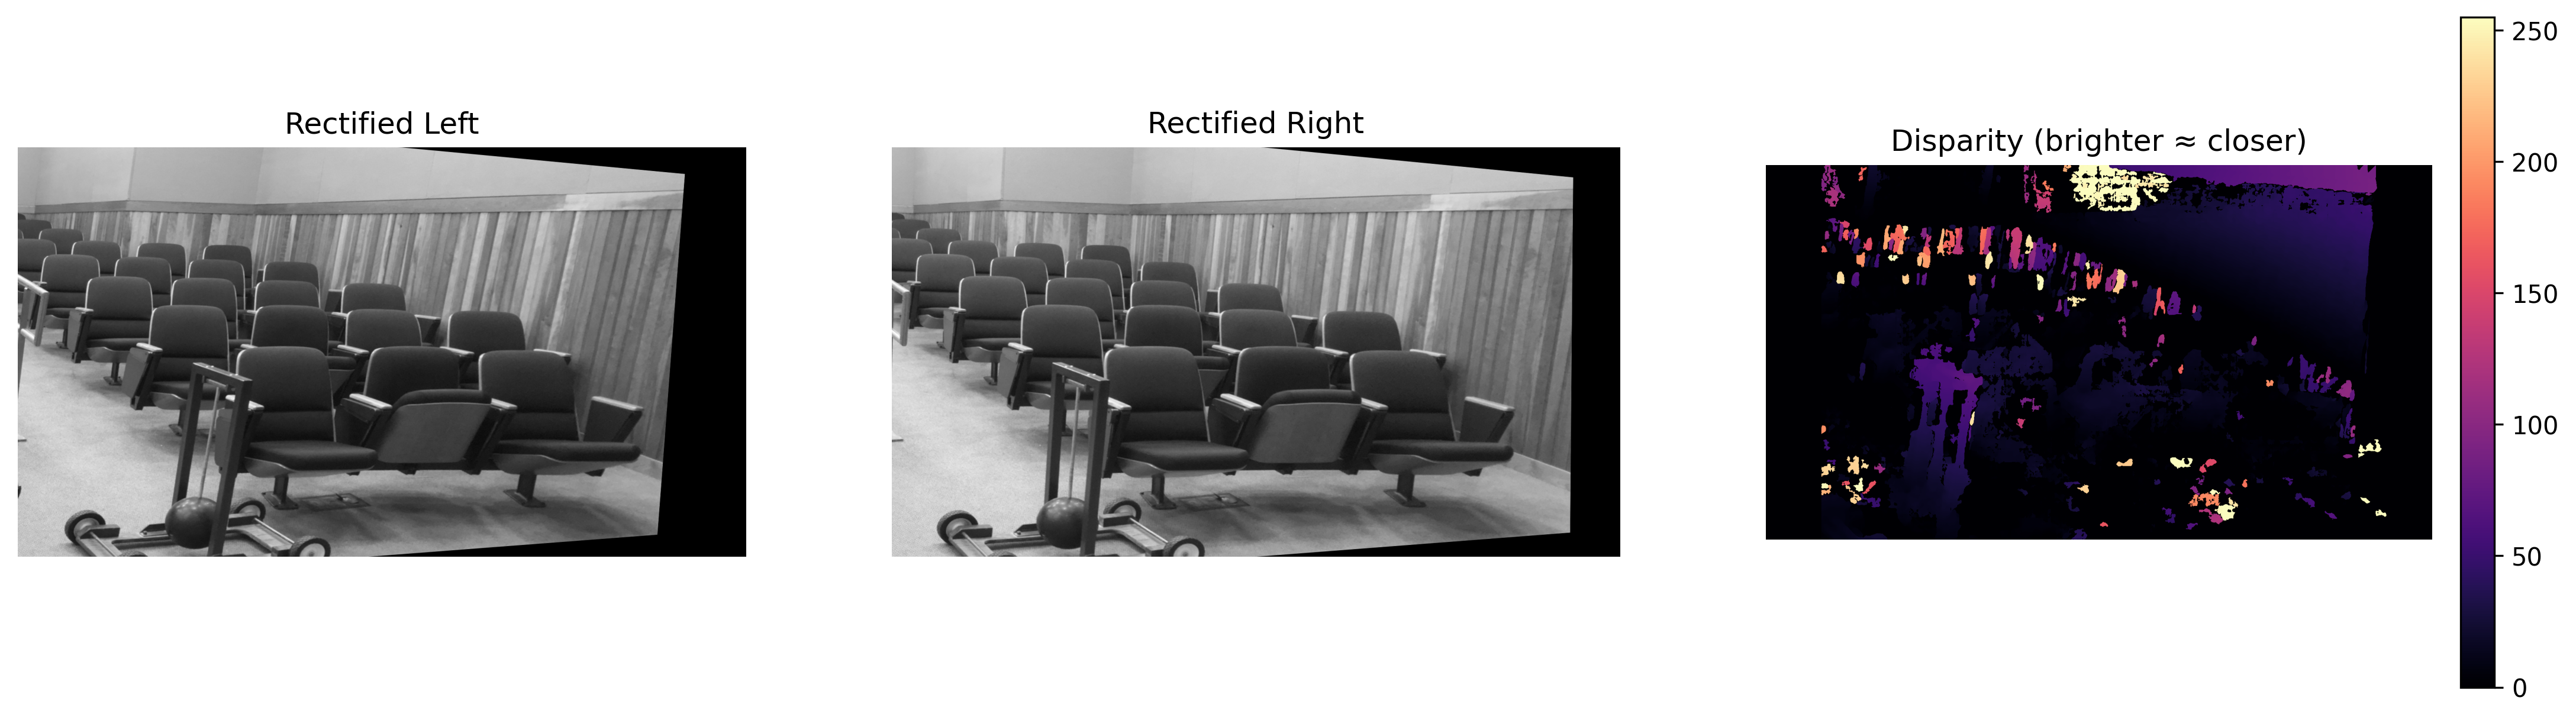
\includegraphics[width=\textwidth]{output/disparity_results.png}
    \caption{Rectified left, rectified right, and SGBM disparity map (brighter $\approx$ closer).}
    \label{fig:disparity}
\end{figure}

\end{document}
